\documentclass[a4paper,11pt]{jsarticle} 
%まず使用するパッケージ
\usepackage{amsmath, amsfonts, amssymb, mathtools, mathrsfs, latexsym}
%mathtoolsを用いたコマンド定義
\DeclarePairedDelimiter{\abs}{\lvert}{\rvert}
\usepackage{nccmath, empheq}

%\usepackage[draft]{graphicx}
\usepackage[dvipdfmx]{graphicx}
\usepackage[dvipdfmx]{color}
\usepackage{here, wrapfig, subcaption}
\usepackage{enumerate, comment, fancyhdr}
\usepackage{otf}

\usepackage{url}
\usepackage{otf}
\usepackage{fancyhdr}
\usepackage{seiritz}
\pagestyle{fancy}
  \cfoot{\thepage}
  \renewcommand{\headrulewidth}{0pt}

\begin{document}
%本文
\begin{titlepage}
  \hfill {最終更新日:\today}
  \begin{center}
    \vspace{\stretch{1}}
    {\Huge\gt テスト演習}\\ \vspace{\baselineskip}
    \textup{\large 実施日:2023年12月23日}\\ \vspace{\stretch{1}}
  \end{center}
  \vfill
  \begin{figure}[H]
    
\includegraphics[width=0.1\textwidth]{../images/qrcode.png}
  \end{figure}
\end{titlepage}

\qPart
%!TEX root = *.tex
%%%%%%%%%%%%%%%%%%
% カウンタのリセット
\setcounter{figure}{0}
% 問題文
図1のように,
傾きの角$30^\circ$のなめらかな斜面上に質量$m$の台車が置かれ,
その台車には軽く伸び縮みしない糸の一端が取り付けられている.
その糸のもうー端は,
斜面の上端に固定された定滑車と,
床と軽いばねでつながれた動滑車を介して,
天井に取り付けられている.
なお,台車,定滑車,動滑車,糸は,すべて同一の鉛直面内にあり,
台車から定滑車までの糸は斜面と平行,
定滑車から動滑車および動滑車から天井までの糸は鉛直で,
糸がたるむことはないものとする.
また,2つの滑車は軽く,なめらかに回るものとする.



台車が静止しているときの位置をつり合いの位置とする.
図1のように,このつり合いの位置から,
斜面の最下点までの距離を$L$とする.
なお,距離$L$,ならびに,台車から定滑車までの距離は,
後述する単振動による台車の振幅に対して,
十分に長いものとする.
また,ばね定数を$k$,重力加速度の大きさを$g$とする.
空気抵抗や摩擦は無視できるものとして,
以下の問いに答えなさい.
ただし,解答に用いる物理量を表す記号は,
問題文中に与えられているもののみとする.


\begin{figure}[H]
  \centering
  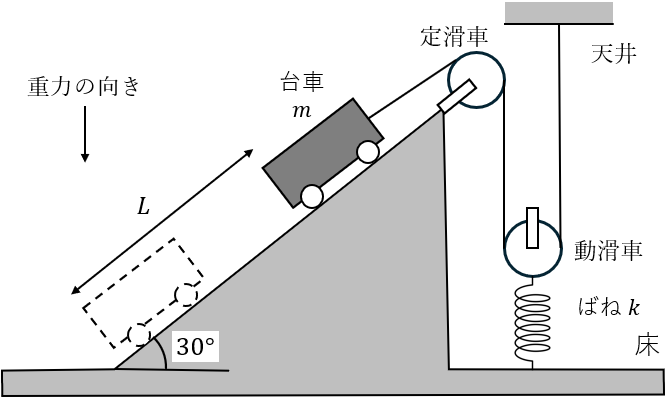
\includegraphics[width=.6\columnwidth]{../graphs/chiba_23_1.png}
  \caption{}
\end{figure}

\begin{enumerate}[(1)]
  \setlength{\leftskip}{-1zw}
  \setlength{\itemindent}{1zw}\setlength{\labelsep}{0.5zw}
  \setlength{\labelwidth}{1zw}\setlength{\leftmargin}{1zw}
  \setlength{\itemsep}{0.5\baselineskip}
  \item つり合いの位置において台車が静止しているときの,糸が天井を引く力の大きさを求めなさい.
  \item つり合いの位置において台車が静止しているときの,ばねの自然長からの伸びを求めなさい.
  \item 台車がつり合いの位置にあるときの,ばねの弾性力による位置エネルギーを求めなさい.
\end{enumerate}



台車の下端を手で支えながら斜面に沿って図1の右上方向にゆっくり移動させ,
ばねが自然長になったところで静かに台車から手をはなしたところ,
台車は斜面に沿って単振動した.



\begin{enumerate}[(1)]
  \setlength{\leftskip}{-1zw}
  \setlength{\itemindent}{1zw}\setlength{\labelsep}{0.5zw}
  \setlength{\labelwidth}{1zw}\setlength{\leftmargin}{1zw}
  \setlength{\itemsep}{0.5\baselineskip}
  \addtocounter{enumi}{3}
  \item 単振動をしている動滑車と台車の振幅をそれぞれ求めなさい.
  \item 単振動をしているときの台車の最大の速さを求めなさい.
  \item この単振動の周期を求めなさい.
\end{enumerate}



ばねが自然長になり台車から手をはなした時刻を$t=0$とする.
手をはなした後,ある時刻で台車に取り付けられた糸を切断する.
なお,糸を切断する直前と直後で,台車の運動エネルギーや位置エネルギーは変化しないものとする.
次の2つの問いについてそれぞれ答えなさい.



\begin{enumerate}[(1)]
  \setlength{\leftskip}{-1zw}
  \setlength{\itemindent}{1zw}\setlength{\labelsep}{0.5zw}
  \setlength{\labelwidth}{1zw}\setlength{\leftmargin}{1zw}
  \setlength{\itemsep}{0.5\baselineskip}
  \addtocounter{enumi}{6}
  \item 手をはなした後,台車がつり合いの位置を2回通過した直後に糸を切断した場合を考える.
  台車は,糸の切断後も,斜面に沿って運動を続けた.
  糸を切断した後に,台車の速さが最初に0になるまでのつり合いの位置からの斜面方向の移動距離と,速さが最初に0になったときの時刻を求めなさい.
  \item 糸の切断時刻を変えることで,台車が斜面の最下点に到達するときの速さを最大にしたい.そのための切断時刻と,台車が斜面の最下点に到達するときの速さを求めなさい.なお,切断時刻は,$t>0$の最も早い時刻とする.
\end{enumerate}







% メモ
\begin{comment}

\end{comment}


%%%%%%%%%%%%%%%%%%


\qPart
%!TEX root = *.tex
%%%%%%%%%%%%%%%%%%
% カウンタのリセット
\setcounter{figure}{0}
% 問題文
図1のように,鉛直上向きで一様な磁束密度$B$の磁場中に,
距離$l$だけ離れた平行な2本の長い導体レールが水平面から角度$\theta\,(0^\circ <\theta <90^\circ)$だけ傾けて固定されている.
導体レールの上端は長さ$l$の細い一様な抵抗線$\text{P}^\prime\text{Q}^\prime$で接続されており,導体レールには,質量$M$,長さ$l$の細い導体棒$\text{PQ}$がそれぞれの導体レールに対して垂直に置かれ,回路を構成している.
この回路に関する以下の問いに答えなさい.
ただし,導体棒と導体レールの間の摩擦や空気抵抗,および抵抗線以外の電気抵抗は無視でき,導体棒は回転しないものとする.
また,回路を流れる電流がつくる磁場は無視できるものとする.
解答においては,抵抗線を$\text{Q}^\prime$から$\text{P}^\prime$へ向かう向きを自由電子(以下,電子と書く)の速度や電流の正の向き,レールに沿って下向きを導体棒の速度の正の向きとしなさい.
また,重力加速度の大きさを$g$とする.電子の電荷を$-e$(ただし,$e>0$),質量を$m$とする.

ある時刻に導体棒は,レールに沿って下向きに速さ$v$で運動していた.


\begin{enumerate}[(1)]
  \setlength{\leftskip}{-1zw}
  \setlength{\itemindent}{1zw}\setlength{\labelsep}{0.5zw}
  \setlength{\labelwidth}{1zw}\setlength{\leftmargin}{1zw}
  \setlength{\itemsep}{0.5\baselineskip}
  \item この導体棒の運動によって発生する誘導起電力を求めなさい.
  \item 誘導起電力によって,抵抗線中に一様な電場が発生した.この電場の大きさを求めなさい.
\end{enumerate}

抵抗線中の電子の運動から抵抗線の抵抗値について考える.
電子の速度を$c$としたとき,電子は速度に比例する抵抗力$-kc$を受けるものとする.
抵抗線中の単位長さあたりの電子の個数を$n$とする.

\begin{enumerate}[(1)]
  \setlength{\leftskip}{-1zw}
  \setlength{\itemindent}{1zw}\setlength{\labelsep}{0.5zw}
  \setlength{\labelwidth}{1zw}\setlength{\leftmargin}{1zw}
  \setlength{\itemsep}{0.5\baselineskip}
  \addtocounter{enumi}{2}
  \item 抵抗線に沿って運動する電子の加速度を$a$として,電子1個に対する運動方程式を$e,\,v,\,B,\,\theta,\,m,\,a,\,k,\,c$を用いて表しなさい.
\end{enumerate}

電子の速度$c$は,十分時間が経った後に速度$c_1$のまま時間変化しなくなった.

\begin{enumerate}[(1)]
  \setlength{\leftskip}{-1zw}
  \setlength{\itemindent}{1zw}\setlength{\labelsep}{0.5zw}
  \setlength{\labelwidth}{1zw}\setlength{\leftmargin}{1zw}
  \setlength{\itemsep}{0.5\baselineskip}
  \addtocounter{enumi}{3}
  \item このときの電子の速度$c_1$を$e,\,v,\,B,\,\theta,\,k$を用いて表しなさい.
  \item 抵抗線中の電子の集団が速度$c_1$で運動することによる電流$I$を$e,\,m,\,k,\,c_1,\,n$のうち必要な記号を用いて表しなさい.
  \item 抵抗線$\text{P}^\prime\text{Q}^\prime$の抵抗値を$e,\,k,\,n,\,l$を用いて表しなさい.
  \item 抵抗線中で電子の速度に比例する抵抗力が単位時間あたりに電子1個に対してする仕事$W$,および単位時間あたりに発生する熱量$J$を,それぞれ$e,\,v,\,B,\,\theta,\,k,\,n,\,l$のうち必要な記号を用いて表しなさい.
\end{enumerate}

次に,図2のように抵抗線を自己インダクタンス$L$のコイルに取り替えた.
時刻$t=0$における導体棒の位置を原点とし,レールに沿って下向きに\x 軸を取った.
時刻$t=0$において静止していた導体棒を静かにはなした後の運動について考える.
導体棒が位置\x にあるとき短い時間$\Delta t$の間の位置の変化を$\Delta x$とし,このときの電流の変化を$\Delta I$とする.
なお,$t=0$において電流は流れていなかった.
また,コイル以外の自己インダクタンスは無視できるものとする.

\begin{enumerate}[(1)]
  \setlength{\leftskip}{-1zw}
  \setlength{\itemindent}{1zw}\setlength{\labelsep}{0.5zw}
  \setlength{\labelwidth}{1zw}\setlength{\leftmargin}{1zw}
  \setlength{\itemsep}{0.5\baselineskip}
  \addtocounter{enumi}{7}
  \item 電流と導体棒の位置の変化は$\Delta I=D\Delta x$と表すことができる.$D$を$B,\,\theta,\,l,\,L$を用いて表しなさい.
\end{enumerate}

前問により,任意の時刻の電流は$I=Dx$と表せることがわかる.

\begin{enumerate}[(1)]
  \setlength{\leftskip}{-1zw}
  \setlength{\itemindent}{1zw}\setlength{\labelsep}{0.5zw}
  \setlength{\labelwidth}{1zw}\setlength{\leftmargin}{1zw}
  \setlength{\itemsep}{0.5\baselineskip}
  \addtocounter{enumi}{8}
  \item 導体棒が位置\x にあるときの導体棒の加速度を$A$として\x 軸方向についての運動方程式を$M,\,A,\,g,\,B,\,\theta,\,l,\,L,\,x$を用いて表しなさい.
  \item 導体棒は単振動をし,導体棒の位置は$x=\alpha +\beta\cos{\omega t}$\,(ただし,$\omega>0$)と表すことができる.$\alpha,\,\beta,\,\omega$をそれぞれ$M,\,g,\,B,\,\theta,\,l,\,L$のうち必要な記号を用いて表しなさい.
  \item 前問のように導体棒の位置が表されるとき,その速度は$-\omega\beta\sin\omega t$と表すことができる.時刻$t$において,コイルに蓄えられているエネルギーと導体棒の力学的エネルギーの合計を求めなさい.ただし,導体棒の位置エネルギーの基準点は$x=0$とする.また,\underline{解答には$M,\,L,\,\alpha,\,\beta,\,\omega$を用いないこと}.
\end{enumerate}

\begin{figure}[H]
  \centering
  \begin{minipage}{.3\columnwidth}
    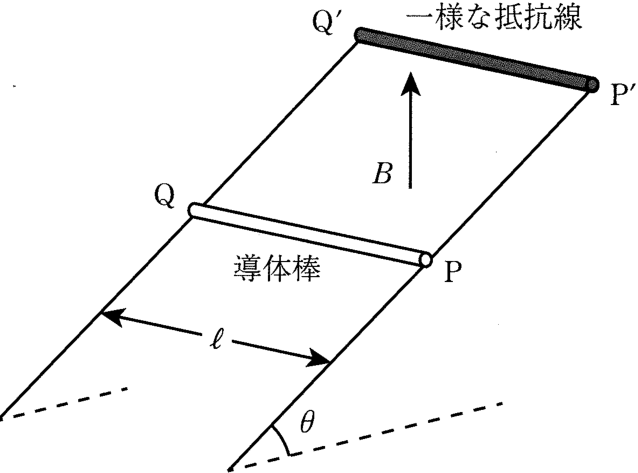
\includegraphics[width=\columnwidth]{../graphs/chiba_23_4-1.png}
    \caption{}
  \end{minipage}
  \hspace{.1\columnwidth}
  \begin{minipage}{.3\columnwidth}
    \centering
    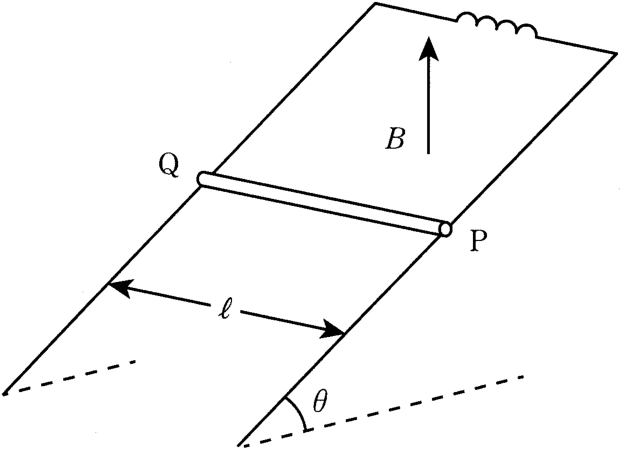
\includegraphics[width=\columnwidth]{../graphs/chiba_23_4-2.png}
    \caption{} 
  \end{minipage}
\end{figure}






% メモ
\begin{comment}

\end{comment}


%%%%%%%%%%%%%%%%%%


\qPart
%!TEX root = *.tex
%%%%%%%%%%%%%%%%%%
% カウンタのリセット
\setcounter{figure}{0}
% 問題文
\noindent\textsf{\bfseries A}\ 
図1のように屈折率$n_1$の媒質\ajRoman{1}と屈折率$n_2$の媒質\ajRoman{2}が水平な境界面で接している.
いま,点A,Bがそれぞれ媒質\ajRoman{1},\ajRoman{2}中にある場合を考える.
点Aは点Bの真上にあり,点A,Bはそれぞれ境界面から距離$d_1$,$d_2$ だけ離れた位置にある.
媒質\ajRoman{2}中の点Bを始点として長さ$l$の棒を水平に置き, 
この棒を点Aから見ることを考える.
棒の他端の位置を点Cとし,点Cを出て点Aに到達する光
が媒質\ajRoman{2}から媒質\ajRoman{1}に入射する際の入射角を$i$,屈折角を$r$とする.棒の長さ$l$は距離$d_1,d_2$に対して十分小さく,
したがって$i,r$も十分小さい.
屈折率は$n_2>n_1$である.
なお,角度はラジアンを単位として表すものとし,
必要であれば,$\theta\,(\theta>0)$が十分小さいときに成り立つ近似式$\sin\theta=\tan\theta=\theta$を用いてよい.



\begin{enumerate}[(1)]
  \setlength{\leftskip}{-1zw}
  \setlength{\itemindent}{1zw}\setlength{\labelsep}{0.5zw}
  \setlength{\labelwidth}{1zw}\setlength{\leftmargin}{1zw}
  \setlength{\itemsep}{0.5\baselineskip}
  \item 点Aから見ると棒の他端は図1の点$\C^\prime$の方向に見える.
  $\B\C^\prime$の長さを点Aから見た棒の見かけの長さとする
  (以下でも同様とする).
  この見かけの長さを$d_1,\,d_2,\,n_1,\,n_2,\,l$を用いて表しなさい.
\end{enumerate}


\begin{enumerate}[(1)]
  \setlength{\leftskip}{-1zw}
  \setlength{\itemindent}{1zw}\setlength{\labelsep}{0.5zw}
  \setlength{\labelwidth}{1zw}\setlength{\leftmargin}{1zw}
  \setlength{\itemsep}{0.5\baselineskip}
  \addtocounter{enumi}{1}
  \item 次に,図2のように長さ$l$の棒を媒質\ajRoman{1}の中に点Aを始点として水平に置いた.点Bから見た棒の見かけの長さを$d_1,\,d_2,\,n_1,\,n_2,\,l$を用いて表しなさい.
\end{enumerate}


\begin{enumerate}[(1)]
  \setlength{\leftskip}{-1zw}
  \setlength{\itemindent}{1zw}\setlength{\labelsep}{0.5zw}
  \setlength{\labelwidth}{1zw}\setlength{\leftmargin}{1zw}
  \setlength{\itemsep}{0.5\baselineskip}
  \addtocounter{enumi}{2}
  \item 棒の長さ$l$をどれだけ長くしても,点Bから見た棒の見かけの長さはある長さ$l_1$より長くなることはなかった.
$l_1$を$d_1,\,d_2,\,n_1,\,n_2,$を用いて表しなさい.ただしこの場合は入射角や屈折角が十分小さいとは限らないことに注意しなさい.
\end{enumerate}



\begin{enumerate}[(1)]
  \setlength{\leftskip}{-1zw}
  \setlength{\itemindent}{1zw}\setlength{\labelsep}{0.5zw}
  \setlength{\labelwidth}{1zw}\setlength{\leftmargin}{1zw}
  \setlength{\itemsep}{0.5\baselineskip}
  \addtocounter{enumi}{3}
  \item 媒質\ajRoman{2}の下に水平な境界面で接している屈折率$n_3\,(n_3>n_2)$の媒質\ajRoman{3}がある場合を考える.
媒質\ajRoman{2}と媒質\ajRoman{3}の境界から距離$d_3$だけ離れた媒質\ajRoman{3}の中に長さ$l$の棒を境界面に水平に置いた.
棒の始点は点Aの真下にある.点Aから見た棒の見かけの長さ$d_1,\,d_2,\,d_3,\,n_1,\,n_2,\,n_3,\,l$を用いて表しなさい.ただし,$l$は$d_3$に比べて十分小さい.
\end{enumerate}



\begin{figure}[H]
  \centering
  \begin{minipage}{.3\columnwidth}
    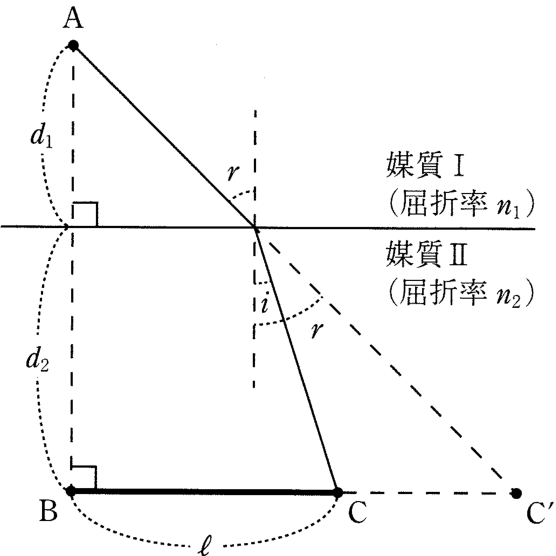
\includegraphics[width=\columnwidth]{../graphs/chiba_23_6-1.png}
    \caption{}
  \end{minipage}
  \hspace{.1\columnwidth}
  \begin{minipage}{.3\columnwidth}
    \centering
    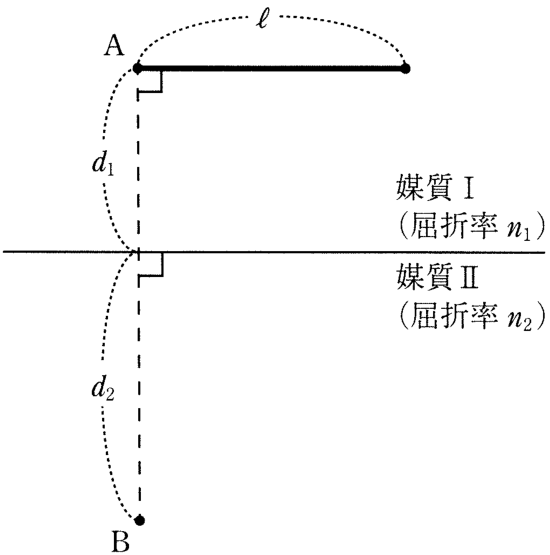
\includegraphics[width=\columnwidth]{../graphs/chiba_23_6-2.png}
    \caption{} 
  \end{minipage}
\end{figure}

\noindent\textsf{\bfseries B}
\ 
反射と屈折の法則は,
「光がある点から別の点まで進むとき,所要時間が最小になるような経路をとる」
というフェルマーの原理から導くことができる.

\begin{enumerate}[(1)]
  \setlength{\leftskip}{-1zw}
  \setlength{\itemindent}{1zw}\setlength{\labelsep}{0.5zw}
  \setlength{\labelwidth}{1zw}\setlength{\leftmargin}{1zw}
  \setlength{\itemsep}{0.5\baselineskip}
  \addtocounter{enumi}{4}
  \item 図3のように\x 軸上に平面鏡を置き,平面鏡に垂直で図の上向きに\y 軸をとる.
  \xy 平面上にある2点A,Bを考え,それぞれの位置を\mbox{$(a_x,\,a_y)$},\mbox{$(b_x,\,b_y)$}とする.
  点Aから出た光が平面鏡で反射して点Bに到達するとき,光は\x 軸上のどこで反射されるかを考える.
  光の道筋は\xy 平面にあるものとし,反射する点の\x 座標を$a_x,\,a_y,\,b_x,\,b_y$を用いて表しなさい.
  ただし,$a_x,\,a_y,\,b_x,\,b_y$はすべて正である.
  \item 次の文章の空欄\BrankNo{(ア)}$\sim$\BrankNo{(カ)}に適切な式を入れなさい.ただし,解答に用いる物理量を表す記号は,以下の文章中に与えられているものとする.\par 
  \vspace{.5\baselineskip}\quad 
  図4のように屈折率$n_1$の媒質\ajRoman{1}と屈折率$n_2$の媒質\ajRoman{2}が水平な境界面で接している.
  媒質\ajRoman{1}中の点Aを出た光が媒質\ajRoman{2}中の点Bに到達する場合を考える.
  光は点Bに到達するまでの時間が最小になるように媒質の境界面上の点を通過する.
  この通過点を点Oとする.以下では屈折率は$n_2>n_1$とする.\par \quad 
  いま,点Oを原点とし,2点A,Bが\xy 面内に含まれる境界面内に\x 軸,
  これと垂直に\y 軸をとる.
  A,Bの座標をそれぞれ$(-a_x,\,a_y)$,$(b_x,\,-b_y)$とする.
  ただし,$a_x,\,a_y,\,b_x,\,b_y$はすべて正である.\par\quad 
  真空中の光の速さを$c$とすると,媒質\ajRoman{1}中の光の速さは\BrankNo{(ア)}であるので,光が経路AOを進むのに要する時間は\BrankNo{(イ)}となる.
  同様にして経路OBを進むのに要する時間も求めることができ,光が経路AOBを進むのに要する時間は\BrankNo{(ウ)}となる.\par\quad 
  次に,光は点Oからわずかにずれた点$\O^\prime\,(\Delta x,\,0)$を通ると仮定する.
  すると,経路$\A\O^\prime$および経路$\O^\prime\B$の距離はそれぞれ\BrankNo{(エ)},\BrankNo{(オ)}となる.
  光が経路AOBに対して経路$\A\O^\prime\B$を進む場合の所要時間の増分を$\Delta t$とする.
  $\Delta x$が十分に小さいため,$(\Delta x)^2$が無視できることを考慮した上で$h$の絶対値が十分に小さいときに成り立つ近似式$\sqrt{1+h}\fallingdotseq 1+\dfrac{h}{2}$を用いることにより,$\dfrac{\Delta t}{\Delta x}$は\BrankNo{(カ)}と求まる.
  ここで,$\dfrac{\Delta t}{\Delta x}=0$となるという条件を課すと,屈折の法則を導くことができる.
\end{enumerate}

\begin{figure}[H]
  \centering
  \begin{minipage}{.3\columnwidth}
    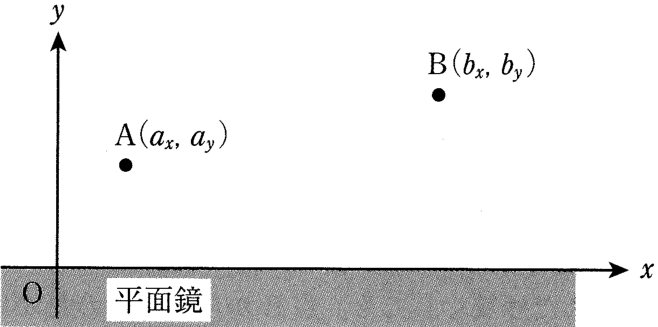
\includegraphics[width=\columnwidth]{../graphs/chiba_23_6-3.png}
    \caption{}
  \end{minipage}
  \hspace{.1\columnwidth}
  \begin{minipage}{.3\columnwidth}
    \centering
    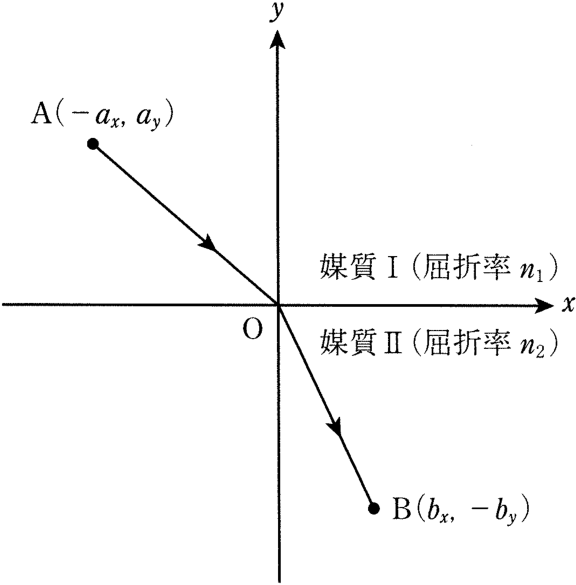
\includegraphics[width=\columnwidth]{../graphs/chiba_23_6-4.png}
    \caption{} 
  \end{minipage}
\end{figure}

% メモ
\begin{comment}

\end{comment}


%%%%%%%%%%%%%%%%%%






\brankPage

\end{document}

